% ----------------------------------------------------------------------------------------%
%	Created by Alessandro with TeXShop						%
%	---->	May 27, 2009										%
%	Compiled with XeLaTeX, on Mac OS X						%
%	Licensed under the Creative Commons Attribution 3.0 Unported	%
%	Share, change, spread, and have fun!						%
%	http://creativecommons.org/licenses/by/3.0/					%
%	You can find more at http://aleplasmati.comuv.com				%
% ----------------------------------------------------------------------------------------%
%  Copyright 2011 Jason Filley
%  I started from Alessandro's template at http://www.cv-templates.info/
%  Multi-page resumes annoy me -- you're too wordy, or 
%  you're listing every product/knowledge you've ever used (if only for 
%  an hour) or overheard someone talking about.  Get to the point.
%
%  http://www.snakelegs.org
%
%  Only tested with XeTeX.  http://scripts.sil.org/xetex
%
%  Same license as above, of course.
%
%  Minor caveat: in the US, at least, employees frequently demand a Microsoft 
%  Word document version of this, but a straight copy/paste loses the small caps.  
%  There are online PDF to Word converters (Rich Text Format), but you may have to 
%  retype a bit, like the section titles.  But it really looks nice as a printed PDF....
% ----------------------------------------------------------------------------------------%

% adjust the points
\documentclass[11pt]{article} %10pt when you add more

\pdfpagewidth 8.5in
\pdfpageheight 11in 

\setlength\topmargin{0in}
\setlength\headheight{0in}
\setlength\headsep{0in}
\setlength\textheight{10in}
\setlength\textwidth{6.5in}
\setlength\oddsidemargin{0in}
\setlength\evensidemargin{0in}
 
%Colors/Graphics
\usepackage{color,graphicx}
\usepackage[usenames,dvipsnames]{xcolor}
\usepackage{pifont}   % for dingbats
\usepackage[hmargin=1.25cm, vmargin=1.5cm]{geometry}               
\usepackage{paralist} % for inparaitem to squish lists

% blue dingbat bullets in address
\definecolor{bullets}{HTML}{104170}
\newcommand{\mybullet}{\mbox{\LARGE\raisebox{+0.2ex}{\tiny{\ding{118}}}}}
\renewcommand{\labelitemi}{\textcolor{bullets}{\mybullet}}

%Fonts and Tweaks for XeLaTeX
\usepackage{fontspec,xltxtra,xunicode}
\usepackage{xeCJK} 
\XeTeXlinebreaklocale "zh" 
\XeTeXlinebreakskip = 0pt plus 1pt 
%Select fonts
\setmainfont[Mapping=tex-text]{Times New Roman} % rm
\setsansfont[Mapping=tex-text]{Arial}           % sf
\setmonofont{Courier New}                       % tt
\setCJKmainfont{NSimSun} %xelatex 新宋体
\setCJKmonofont{Microsoft YaHei}  %xelatex 微软雅黑


\defaultfontfeatures{Mapping=tex-text}
%\setromanfont{Calluna}        %http://www.josbuivenga.demon.nl/calluna.html
	% n.b.: no italics in free version of Calluna / regular face only
%\setsansfont{Goudy Trajan}    %http://castletype.com/html/tipoteca/goudy-trajan-regular.html
%\setmonofont[Scale=MatchLowercase]{Inconsolata} %http://www.levien.com/type/myfonts/inconsolata.html

%Setup hyperref package, and colours for links, text and headings
\usepackage{hyperref}
\definecolor{linkcolour}{HTML}{000000}	% change if you intend for it to be read
	% in a viewer, as opposed to being printed.
\definecolor{text1}{HTML}{000000}		
\definecolor{headings}{HTML}{701112} 	% dark red

\hypersetup{colorlinks,breaklinks,
			urlcolor=linkcolour, 
			linkcolor=linkcolour}

\usepackage{fancyhdr}				%custom footer
\pagestyle{fancy}
\fancyhf{}

%\rfoot{\color{headings}
%{\sffamily Copyright \copyright~2013 Jibin Ou. All rights reserved.}}
	
\renewcommand{\headrulewidth}{0pt}
\usepackage{titlesec}				%custom \section
\usepackage{graphicx}
\usepackage{adjustbox}

\titleformat{\section}
	{\color{headings}
		\scshape\Large\raggedright}{}{0em}{}[\color{black}\titlerule]
\titlespacing{\section}{0pt}{0pt}{5pt}

\begin{document}

%START of left-hand side minipage
\begin{minipage}[t]{0.5\textwidth} 
\vspace{0pt}	%trick
\adjustbox{valign=t}{\begin{minipage}{0.25\linewidth}
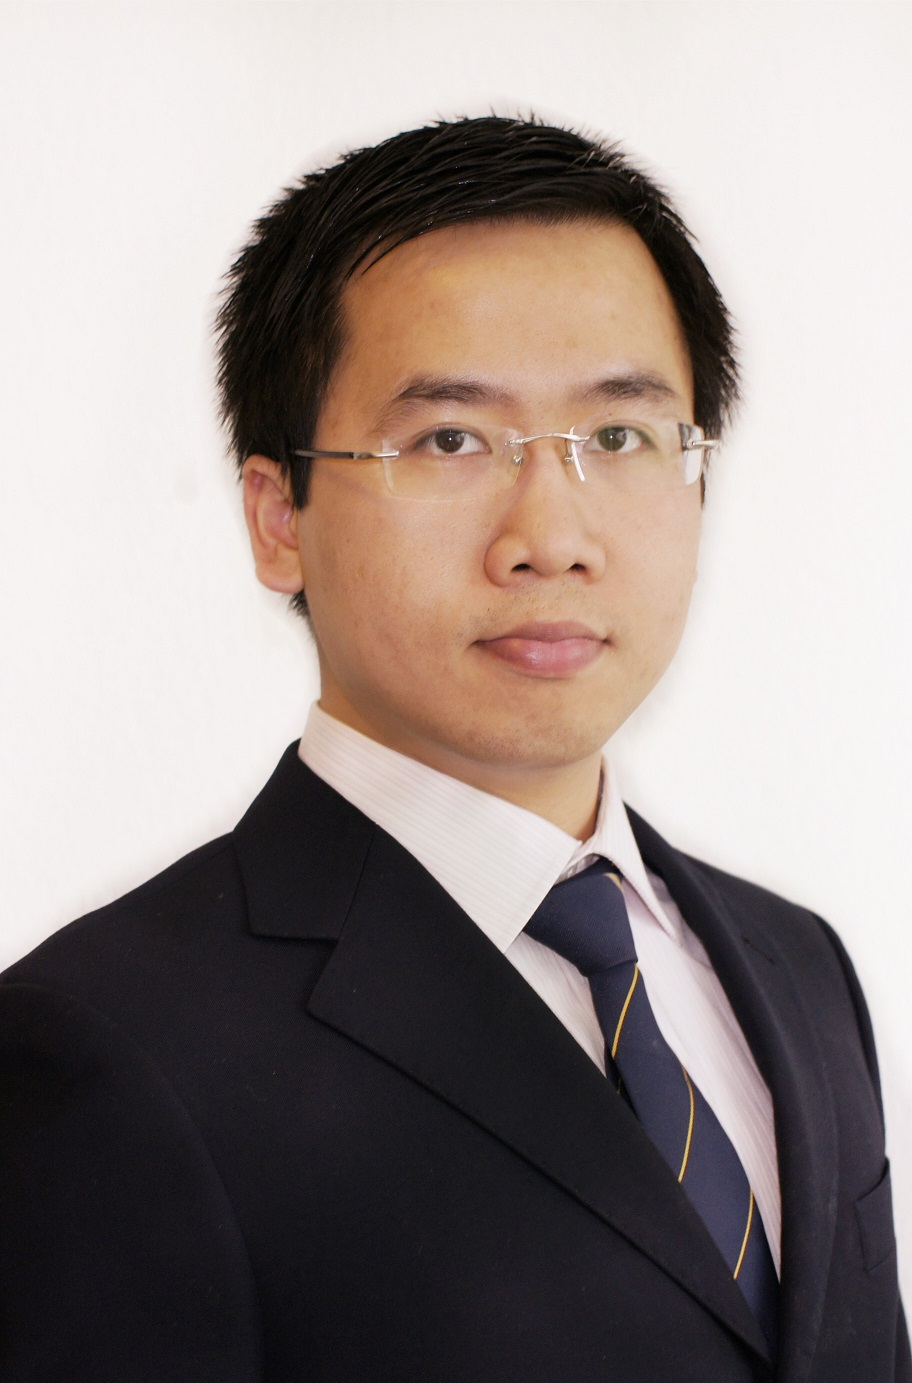
\includegraphics[width=1\linewidth]{photo.jpg}
\end{minipage}}%
\hfill
\adjustbox{valign=t}{
\begin{minipage}[t]{0.70\textwidth} 
\color{text1} % set text color for the whole doc
{\fontsize{30}{30}\selectfont\color{headings} 欧继斌}\\
现居地: 上海市嘉定区\\
出生年月: 1987年9月 \\
电话: +86-1359-0517-629\\
\href{mailto:jibin.ou@outlook.com}{邮件: jibin.ou@outlook.com}\\
{项目网址: http://insyncim64.github.io}\\
% {常用博客: http://www.jibinou.cn} \\
方向: 软件, 算法开发工程师\\
\color{text1}
\end{minipage}}
\newline
% \section{求职意向}
% 在上海的互联网企业的研发岗位, 入职时间2016年9月\\
 
\section{教育背景}
\normalsize{研究生, 媒体信息学专业, 亚琛工业大学\hfill10.2010--04.2014}\\
\small{亚琛, 德国}\\\par
\normalsize{访问学生, 计算机系, 苏黎世理工大学\hfill07.2013--04.2014}\\
\small{苏黎世, 瑞士}\\\par
\normalsize{本科, 信息与计算科学专业, 中山大学\hfill09.2006--06.2010}\\
\small{广州, 中国}\\\par
\normalsize{交换学生, 数学系, 华东师范大学\hfill02.2009--06.2009}\\
\small{上海, 中国}\\\par

\section{工作经验}
% use empty [] after the first item to suppress the bullet
\normalsize{霍尼韦尔综合科技, 软件工程师\hfill10.2016--至今\\
\small{上海}\\
\begin{inparaitem}
	\item 参与美国, 德国和印度团队, 共同进行软件研发;
	\newline
	\item 管理与维护Movilizer解决方案中国区的服务器;
	\newline
	\item 参与进行本地软件相关的创新项目;
\end{inparaitem}}
\\\par

\normalsize{霍尼韦尔, 自动化控制系统集团, 软件工程师\hfill01.2015--09.2016\\
\small{曼海姆, 德国}\\
\begin{inparaitem}
	\item 负责基于Swing和JavaFX的桌面客户端开发;
	\newline
	\item 基于J2ME, Raspberry Pi的嵌入式客户端开发;
	\newline
	\item 服务器端程序开发, 使用到Apache Cassandra分布式服务器, Spring, JAXB及JavaCC等框架;
\end{inparaitem}}
\\\par

\normalsize{苏黎世理工大学, 人机交互实验室, 研究助理\hfill04.2014--12.2014\\
\small{苏黎世, 瑞士}\\
\begin{inparaitem}
	\item 研究下一代可视化编程环境;主持用户调研、用户实验, 及分析调研数据, 发表论文;
\end{inparaitem}}
\\\par

\normalsize{研发实习生, 整车装配验证组, 宝马集团\hfill01.2013--06.2013\\
\small{慕尼黑, 德国}\\
\begin{inparaitem}
	\item 独立完成了基于iPad, Windows平板和Anoto笔等设备的, 用于整车装配验证的远程协作系统原型, 此系统将部署于分布全球各地的生产部, 方便工程师之间的沟通.
\end{inparaitem}}
\\\par

\normalsize{研究助理, Fraunhofer应用信息技术研究院}\\
\small{波恩, 德国}\hfill\normalsize{08.2011--07.2012}\\
\small{
\begin{inparaitem}
	\item 开发实时家电监控系统;
	\newline
	\item 研究如何使用传感器融合, WiFi信号三角定位等方法提高移动电话定位的准确性.
\end{inparaitem}}
\\\par

%\normalsize{实习生, 伊罗奇国际贸易有限公司\hfill04.2009--08.2009}\\
%\small{上海, 中国\\ 
%\begin{inparaitem}
%	\item 为上海办事处的物流组开发协作平台;
%	\newline
%	\item 对公司服务器进行日常维护, 为员工提供IT培训.
%\end{inparaitem}}
%\\\par


\end{minipage} %END of left-hand side minipage
\hfill
\begin{minipage}[t]{0.44\textwidth} %START of right-hand side minipage

\vspace{0pt} %trick for alignment
	
\section{相关项目}
%\normalsize{北上广一二手房成交查询\hfill01.2016--至今}\\
%\small 私人项目, 曼海姆, 德国\\
%\small
%\begin{inparaitem} 
%\item 使用爬虫抓取每天成交纪录, 提供查询与分析功能\\
%\item 基于SpringMVC, MongoDB的后端, 前端使用Angular 2, Bootstrap和TypeScript, 爬虫使用基于Selenium的爬虫, 方便抓取webapp信息.\\
%\end{inparaitem}
%\par

\normalsize{基于OBD接口数据的汽车检测\hfill09.2017--至今}\\
\small 霍尼韦尔, 上海\\
\small
\begin{inparaitem} 
\item 基于OBD接口数据的二手车诊断服务, 为部门内的新2B业务;\\
\item 负责云平台搭建, 后端团队为5人规模. 使用go语言, beego框架, postgresSQL作用户数据的管理, Cassandra数据库存储OBD元数据.
\end{inparaitem}
\\\par 

\normalsize{霍尼韦尔互联卡车项目\hfill12.2016--08.2017}\\
\small 霍尼韦尔, 上海\\
\small
\begin{inparaitem} 
\item 基于传感器, 网关, 云与移动解决方案的物联网项目;\\
\item 参与移动端与桌面端基于Movilizer解决方案的应用程序的开发.
\end{inparaitem}
\\\par 

\normalsize{基于结构光的移动快递包裹体积测量\hfill04.2017--至今}\\
\small 霍尼韦尔, 上海\\
\small
\begin{inparaitem} 
\item 使用基于结构光的深度摄像头, 利用Ransac算法发现立方体再测量出其体积;\\
\item 基于Windows 10平板,使用RealSense SDK开发出内部使用的原型产品.
\end{inparaitem}
\\\par

\normalsize{基于深度学习的超市果蔬称重电子秤\hfill04.2017--至今}\\
\small 霍尼韦尔, 上海\\
\small
\begin{inparaitem} 
\item 使用Tensorflow框架与Inception-v3模型, 对从ImageNet筛选出来的水果蔬菜数据集进行训练;\\
\item 对151种水果蔬菜的分类Top-5成功率为3.37\%, 使用Raspberry Pi 3B制作的产品原型可达到0.5FPS.
\end{inparaitem}
\\\par 

\normalsize{堆内存的可视化和实时操作\hfill07.2013--03.2014}\\
\small 苏黎世理工大学, 苏黎世, 瑞士\\
\small
\begin{inparaitem} 
\item 以图的形式将堆内存的逻辑关系呈现, 提供基于手势和笔触的交互, 可对内存对象进行操作, 由两教授共同指导的硕士论文\\
\item 建立基础的数学模型, 可供建立手势操作和内存遍历之间的逻辑关系, 为内存的可视化或操作提供基础;\\
\item 独立设计和开发信息可视化组件, 内存遍历模块使用Eclipse RCP平台实现, 可视化模块使用WPF实现.\\
\end{inparaitem}
\\\par 

%\normalsize{WeAnnotate: 带有分享功能的PDF文档阅读器}\\
%\small 亚琛工业大学, 亚琛, 德国\hfill\normalsize{04.2012--07.2012}\\
%\small
%\begin{inparaitem} 
%\item 参与开发基于安卓平板的App的PDF阅读器, 可以便捷地注释PDF文档并提供注释分享功能;\\
%\item 作为项目组长制定项目计划, 解决项目中的重点技术问题, 包括如何在Android系统上显示和注释PDF文档, 并将注释持久化等问题;\\
%\end{inparaitem}
%\par 

%\normalsize{基于位置信息的撞球游戏\hfill01.2012--04.2012}\\
%\small{Fraunhofer应用信息技术研究院, 波恩, 德国}\\
%\small
%\begin{inparaitem} 
%\item {设计并开发了使用用户的绝对位置去控制的经典撞球游戏;}\\
%\item {独立实施了基于高通Alljoyn框架的WiFi点对点传输, 使移动电话可以无访问接入点的情况下进行通信;}\\
%\item {测试并对比了不同的定位技术, 为游戏的技术层面提供可行的定位方案.}\\
%\end{inparaitem}
%\par

\section{获奖及论文} 
\begin{inparaitem}
\item \normalsize{论文《An Interactive System for Data Structure Development》,  Jibin Ou, Martin Vechev, Otmar Hilliges, ACM CHI会议, \hfill\normalsize04.2015\\\small{首尔, 韩国}\par}
\item \normalsize{获得IDEA联盟学生研究奖学金\hfill\normalsize07.2013\\\small{苏黎世, 瑞士}\par}
\end{inparaitem}
\par

\section{语言及计算机技能}
\normalsize
英语: 托福95/120; 德语: DSM B1等级, 熟练水平; 
\\ 粤语: 母语水平\\
编程语言和框架: 
\textbf{语言: }Java, Go, Python\\
\textbf{框架与工具: }Tensorflow, Keras, Spring\\
\textbf{相关课程:} 机器学习, 人机交互和程序分析\\


\end{minipage} %END of right-hand side minipage
\end{document}  